%% ============================================================================
%%  IEEE Transactions on Neural Networks and Learning Systems (TNNLS)
%%  Two-column journal version.
%%
%%  Compile with the genuine IEEEtran.cls (ships with TeX Live / MiKTeX, and is
%%  the default on Overleaf's "IEEE Transactions" template):
%%      pdflatex main_ieee
%%      bibtex   main_ieee
%%      pdflatex main_ieee
%%      pdflatex main_ieee
%% ============================================================================
\documentclass[journal]{IEEEtran}

% --- math / graphics / tables ----------------------------------------------
\usepackage{amsmath,amssymb,mathtools}
\usepackage{graphicx}
\graphicspath{{figures/}}
\usepackage{booktabs}
\usepackage{array}
\usepackage[caption=false,font=footnotesize]{subfig}
\usepackage{algorithm}
\usepackage{algpseudocode}
\usepackage{xcolor}

% --- hyperlinks / cross-references (load hyperref before cleveref) ----------
\usepackage[hidelinks]{hyperref}
\usepackage{cleveref}

% --- schematic --------------------------------------------------------------
\usepackage{tikz}
\usetikzlibrary{arrows.meta,calc}

% --- IEEEtran-friendly float spacing ---------------------------------------
\renewcommand{\arraystretch}{1.15}

% --- convenience macros (keep notation identical to the code) ---------------
\newcommand{\vth}{v_{\mathrm{thresh}}}
\newcommand{\vr}{v_{\mathrm{rest}}}
\newcommand{\vre}{v_{\mathrm{reset}}}
\newcommand{\vmin}{v_{\min}}
\newcommand{\teff}{\theta_{\mathrm{eff}}}
\newcommand{\rinf}{r_{\infty}}
\newcommand{\Gb}{G_{b}}
\newcommand{\Gbase}{G_{\mathrm{base}}}
\newcommand{\Gdyn}{G_{\mathrm{dyn}}}
\newcommand{\Jdb}{J_{\mathrm{DB}}}
\newcommand{\code}[1]{\texttt{#1}}

\begin{document}

\title{A Mathematically Consistent, Nengo-Compatible Reference Implementation
of HyperLIF and Adaptive HyperLIF Neurons: Continuous Gate-State Dynamics,
Exact Validation, and a Bridge to Gate-State Residual Decoding}

\author{Adaptive~HyperLIF~/~Nengo~Research~Project%
\thanks{Companion implementation and validation study to the Adaptive HyperLIF
theory manuscript~\cite{hyperlif_theory}. This manuscript is submitted for
review; author identities and affiliations have been anonymized for
double-blind peer review.}}

\markboth{IEEE Transactions on Neural Networks and Learning Systems}%
{Anonymous \MakeLowercase{\textit{et al.}}: Nengo-Compatible Reference Implementation of HyperLIF Neurons}

\maketitle

\begin{abstract}
The leaky integrate-and-fire (LIF) neuron resets its membrane potential
discontinuously at threshold, which is convenient for simulation but makes the
state evolution non-smooth and obscures the sub-threshold ``readiness'' state of the
neuron. The companion theory manuscript~\cite{hyperlif_theory} replaces the
hard reset with a continuous, gate-controlled discharge, yielding the
\emph{HyperLIF} neuron and its input-stabilized variant, \emph{Adaptive
HyperLIF}. This paper contributes a clean, self-contained, and rigorously
validated reference implementation of those neurons that is compatible with the
Neural Engineering Framework toolkit Nengo~\cite{bekolay2014nengo}. We restate
the implemented equations exactly as coded, expose two numerical stepping
schemes---an explicit-Euler scheme matching the Julia reference and an
exponential-Euler scheme used by the Nengo port---and analyze their accuracy and
stability against a fine Runge--Kutta reference. A frozen-open-gate equilibrium
analysis gives the branch estimate
$\Jdb=(\vth-\gamma)(1+\tau\Gb)=2.4$ for the reference parameters and the branch
voltage $v^\ast=J/(1+\tau\Gb)$; the voltage prediction matches the simulated
high-drive latch (e.g.\ $v^\ast=1.3333$ predicted and observed at $J=4$). The
adaptive conductance law bounds the positive-drive, $r=1$ asymptotic branch below
the gate knee when $\beta>1/(\tau(\vth-\gamma))=62.5$ (here $\beta=80$). This
changes the high-drive regime but is not a global-stability or firing theorem.
We further show that the standalone exponential stepping
and the Nengo custom-neuron stepping agree to floating-point exactness (voltage
and gate RMSE $=0$, zero event-timing mismatch) across two stimulus protocols
and both models, because both call an identical numerical kernel. Finally, we
interpret the continuous reset gate as a decodable readiness-to-fire signal and
outline---explicitly as future work---how it can serve as a residual feature for
Nengo-based adaptive quaternion attitude control. All figures, tables, and
claims are reproducible from the included code and data.
\end{abstract}

\begin{IEEEkeywords}
Spiking neural networks, leaky integrate-and-fire model, continuous reset,
depolarization block, Neural Engineering Framework, Nengo, numerical
integration, neuromorphic computing.
\end{IEEEkeywords}

% ===========================================================================
\section{Introduction}\label{sec:intro}
% ===========================================================================
\IEEEPARstart{T}{he} discontinuous threshold-and-reset rule of the LIF
neuron~\cite{lapicque1907} makes spike generation a hybrid (non-smooth)
dynamical process. This is the root cause of two practical difficulties. First,
the reset map is not differentiable, so gradient-based training of spiking
networks must either approximate the missing derivative with surrogate
gradients~\cite{neftci2019surrogate} or handle spike events explicitly with
specialized adjoint machinery~\cite{wunderlich2021eventprop}. Second, the
instantaneous jump discards information: the moment the membrane reaches
threshold, its trajectory is overwritten, leaving only the emitted event as an
observable. The continuous-reset \emph{HyperLIF} family introduced in the
companion theory manuscript~\cite{hyperlif_theory} removes the discontinuity by
modeling the reset as a fast but smooth, gate-controlled discharge, producing a
continuous-state ordinary differential equation (ODE) system with an explicit,
interpretable internal gate state $r(t)$. The binary event observable remains
non-differentiable; event-dependent losses require a surrogate or an explicit
event-time derivative. Adaptive HyperLIF also contains a non-smooth $|J|$ term
at $J=0$ unless it is regularized.

Theory and benchmark performance for the HyperLIF family are reported in
\cite{hyperlif_theory}. The present paper addresses a complementary and equally
important question for downstream use: \emph{can these continuous-reset neurons
be implemented as a clean, equation-faithful, and numerically validated
component of a standard neural-engineering workflow?} We answer this
affirmatively by building a small reference package that (i) implements LIF,
HyperLIF, and Adaptive HyperLIF from a single mathematical specification, (ii)
ports HyperLIF and Adaptive HyperLIF to Nengo~\cite{bekolay2014nengo} as custom
\code{NeuronType} classes with probeable continuous state, and (iii) validates
the port against the standalone implementation to floating-point exactness. The
Neural Engineering Framework (NEF)~\cite{eliasmith2003neural} that underlies
Nengo provides a principled route from encoded stimuli to decoded estimates, and
has been used for closed-loop adaptive robot control~\cite{dewolf2016reach}; a
validated HyperLIF \code{NeuronType} is the prerequisite for using the
continuous gate state inside that workflow.

\subsection*{Contributions}
This paper makes the following contributions.
\begin{enumerate}
  \item A single-source, equation-faithful reference implementation of LIF,
  HyperLIF, and Adaptive HyperLIF, with every manuscript equation traceable to
  specific lines of code (\Cref{sec:formulation,sec:lif,sec:hyperlif,sec:adaptive}).
  \item A closed-form characterization of the frozen open-gate equilibrium:
  the branch estimate $\Jdb=(\vth-\gamma)(1+\tau\Gb)$ and branch voltage
  $v^\ast=J/(1+\tau\Gb)$, checked against high-drive simulation, and the
  condition $\beta>1/(\tau(\vth-\gamma))$ under which the adaptive positive-drive,
  $r=1$ asymptote lies below the gate knee
  (\Cref{sec:hyperlif,sec:adaptive,sec:results-fi}).
  \item An analysis of the two discrete stepping schemes (explicit-Euler vs.\
  exponential-Euler) against a Runge--Kutta reference, quantifying convergence
  and contractivity of its frozen scalar exponential substep
  (\Cref{sec:integration,sec:results-integration}).
  \item A demonstration that the Nengo port reproduces the standalone
  exponential stepping \emph{exactly} (voltage/gate RMSE $=0$, zero event
  mismatch) across protocols and models, with an explanation grounded in a
  shared numerical kernel (\Cref{sec:nengo,sec:results-parity}).
  \item An interpretation of the reset gate as a decodable readiness-to-fire
  signal, and an explicitly-labeled future-work bridge to gate-state residual
  decoding for quaternion attitude control
  (\Cref{sec:readiness,sec:bridge}).
\end{enumerate}

% ===========================================================================
\section{Motivation and Background}\label{sec:background}
% ===========================================================================
\subsection{From Hard Reset to Continuous Reset}
A standard LIF neuron integrates its input and, upon crossing $\vth$, is reset
to $\vre$ instantaneously. The companion theory~\cite{hyperlif_theory} reframes
this jump as the standard-real projection of an infinitesimal-time discharge,
producing a stiff two-time-scale ODE in which a fast gate variable $r(t)$
mediates a continuous reset conductance. Enforcing continuity exposes dynamical
regimes that the idealized hybrid abstraction hides---most notably a
depolarization block (DB), a silent depolarized mode under sustained strong
drive that is well documented in biophysical
models~\cite{bianchi2012db,dovzhenok2012db} and is the continuous-system
resolution of a Zeno-like accumulation of reset events~\cite{zhang2001zeno}. The
Adaptive HyperLIF changes the high-drive branch over the intended operating range by
scaling the reset conductance with input magnitude. We take these models as
given and focus on a faithful, validated realization.

\subsection{Why Nengo Compatibility Matters}
Nengo~\cite{bekolay2014nengo} implements the NEF~\cite{eliasmith2003neural}:
populations of neurons encode signals through tuning curves and decode them
through learned linear weights. Implementing HyperLIF as a Nengo
\code{NeuronType} places the continuous-reset neuron inside this standard
ecosystem---probeable state, calibrated gains/biases, and ensemble decoding---so
that the gate state can be used as a decodable feature alongside spikes and
voltage. Because NEF-based spiking controllers have been demonstrated for
adaptive robotic control~\cite{dewolf2016reach}, a validated port is the natural
substrate for the attitude-control direction discussed in \Cref{sec:bridge}.

\subsection{Notation}
\Cref{tab:notation} fixes the notation, which is identical to the symbols used
in the code and in \cite{hyperlif_theory}. Unless stated otherwise we use the
normalized convention $\vr=\vre=0$, $\vth=1$, so $J$ and the conductance $G$ are
dimensionless relative to the leak term.

\begin{table}[t]
\centering
\caption{Notation used throughout the paper.}
\label{tab:notation}
\footnotesize
\begin{tabular}{@{}ll@{}}
\toprule
Symbol & Meaning \\
\midrule
$v(t)$ & Membrane voltage (normalized) \\
$r(t)\in[0,1]$ & Continuous reset gate (fast activation-like proxy) \\
$J\;(=I_{\mathrm{in}})$ & Net input current / drive (normalized) \\
$\tau,\tau_r$ & Membrane and gate time constants ($\tau_r\ll\tau$) \\
$\vr,\vre,\vth$ & Rest, reset, threshold voltages \\
$\sigma(\cdot)$ & Logistic gate detector, steepness $\alpha$ \\
$\gamma,\teff$ & Hysteresis and effective threshold $\teff=\vth-\gamma r$ \\
$\Gb$ & Fixed reset gain (baseline HyperLIF) \\
$\Gbase,\beta$ & Baseline gain and adaptive scaling (Adaptive) \\
$G(r,J)$ & Reset conductance scale; $\Gb r^2$ or $(\Gbase+\beta|J|)r^2$ \\
$\Gdyn$ & Adaptive conductance scale $\Gbase+\beta|J|$ \\
$\lambda$ & Membrane relaxation rate $1/\tau + G$ \\
$\Jdb$ & Frozen-open-gate DB branch estimate \\
$\Delta t$ & Simulation time step \\
\bottomrule
\end{tabular}
\end{table}

% ===========================================================================
\section{Mathematical Formulation}\label{sec:formulation}
% ===========================================================================
All three neuron models share the membrane/leak structure; they differ in how
the reset is realized. We state each model exactly as implemented. A compact
qualitative comparison is given in \Cref{tab:modelcompare}, and the default
parameters (reflected directly from the parameter dataclasses) in
\Cref{tab:params}.

\begin{table*}[t]
\centering
\caption{Qualitative comparison of the three neuron models in the reference implementation.}
\label{tab:modelcompare}
\begin{tabular}{@{}p{0.20\textwidth}p{0.22\textwidth}p{0.24\textwidth}p{0.26\textwidth}@{}}
\toprule
Property & LIF & HyperLIF & Adaptive HyperLIF \\
\midrule
State variables & $\{v\}$ & $\{v,r\}$ & $\{v,r\}$ \\
Reset mechanism & hard jump to $\vre$ & gate conductance $\Gb r^2$ & input-modulated $(\Gbase+\beta|J|)r^2$ \\
Threshold event & discontinuous & smooth crossing & smooth crossing \\
Continuous \& differentiable & no (hybrid) & yes & yes \\
Refractory handling & explicit $\tau_{\mathrm{ref}}$ & gate hysteresis $\gamma$ & gate hysteresis $\gamma$ \\
High-drive behaviour & increasing firing & high-voltage latch & bounded subthreshold dynamics \\
Nengo \code{NeuronType} & (built-in) & \code{HyperLIFNengo} & \code{AdaptiveHyperLIFNengo} \\
\bottomrule
\end{tabular}
\end{table*}

% ---------------------------------------------------------------------------
\subsection{LIF Baseline}\label{sec:lif}
The baseline LIF membrane obeys
\begin{equation}
  \frac{dv}{dt} = \frac{-(v-\vr) + J}{\tau}. \label{eq:lif-ode}
\end{equation}
For a sub-threshold step the implementation advances the membrane with the exact
linear update
\begin{equation}
  v_{k+1} = (\vr + J) + \big(v_k - \vr - J\big)\,e^{-\Delta t/\tau},
  \label{eq:lif-update}
\end{equation}
which is the closed-form solution of \cref{eq:lif-ode} for constant $J$. If the
membrane crosses threshold from below, $v_k<\vth\le v_{k+1}$, the neuron emits an
event of magnitude $A/\Delta t$ (Nengo's spike convention), is reset to $\vre$,
and enters a refractory interval $\tau_{\mathrm{ref}}$ during which the voltage
is held at $\vre$. The voltage is clamped from below at $\vmin$. This is a
deliberately minimal hard-reset reference for figures and decoding comparisons,
not a replacement for Nengo's production LIF.

% ---------------------------------------------------------------------------
\subsection{HyperLIF Model}\label{sec:hyperlif}
HyperLIF augments the membrane with a continuous reset gate $r(t)\in[0,1]$. The
gate detector is a steep logistic with effective threshold
$\teff=\vth-\gamma r$ (a hysteresis that lowers the threshold as the gate opens):
\begin{align}
  \teff &= \vth - \gamma r, \label{eq:theta}\\
  \rinf &= \sigma\!\big(\alpha (v-\teff)\big), \quad
  \sigma(x) = \frac{1}{1+e^{-x}}. \label{eq:sigmoid}
\end{align}
The two-state continuous-time dynamics are
\begin{align}
  \frac{dr}{dt} &= \frac{\rinf - r}{\tau_r}, \label{eq:gate-ode}\\
  \frac{dv}{dt} &= \frac{-(v-\vr)+J}{\tau} - G(r)\,(v-\vre), \;\;
  G(r) = \Gb\, r^2. \label{eq:hyperlif-ode}
\end{align}
The reset conductance $G(r)=\Gb r^2$ is quadratic in the gate so that
$\partial G/\partial r = 0$ at gate onset, preserving a sharp, LIF-like upstroke
until the gate commits~\cite{hyperlif_theory}. Crucially, \emph{there is no hard
reset}: \cref{eq:hyperlif-ode} pulls the membrane toward $\vre$ continuously
through $G(r)$. Events are emitted for readout only, on an upward crossing of an
event level $v_{\mathrm{event}}$ (by default $\vth$), and do not alter the state.

\paragraph{Open-gate equilibrium and the depolarization block}
Setting $dv/dt=0$ in \cref{eq:hyperlif-ode} for a frozen gate value $r$ and
constant $J$ gives the membrane equilibrium
\begin{equation}
  v^\ast(r) = \frac{\vr + J + \tau\,G\,\vre}{1 + \tau\,G}, \qquad G=\Gb r^2,
  \label{eq:vstar}
\end{equation}
i.e.\ the drive divided by the total (leak plus reset) conductance. Under strong
sustained drive the gate saturates open ($r\to 1$). In the normalized convention
$v^\ast(1)=J/(1+\tau\Gb)$. Equating this \emph{frozen open-gate branch}
with the gate knee $\teff(1)=\vth-\gamma$ gives the useful branch estimate
$v^\ast(1)\ge \vth-\gamma$. Solving for the corresponding current,
\begin{equation}
  \boxed{\;\Jdb = (\vth-\gamma)\,(1+\tau\Gb) - \vr - \tau\Gb\,\vre.\;}
  \label{eq:jdb}
\end{equation}
For the reference parameters ($\vth=1,\gamma=0.2,\tau=0.02,\Gb=100$),
\cref{eq:jdb} gives $\Jdb=0.8\times 3 = 2.4$, and the latched voltage at, e.g.,
$J=4$ is $v^\ast(1)=4/3=1.3333$. \Cref{sec:results-fi} confirms both numbers
against simulation.

% ---------------------------------------------------------------------------
\subsection{Adaptive HyperLIF Model}\label{sec:adaptive}
Adaptive HyperLIF keeps \cref{eq:theta,eq:sigmoid,eq:gate-ode} unchanged and
replaces the fixed reset gain by an input-dependent conductance scale,
\begin{equation}
  \Gdyn = \Gbase + \beta\,|J|, \quad
  G(r,J) = \Gdyn\, r^2 = (\Gbase + \beta\,|J|)\, r^2,
  \label{eq:adaptive-gain}
\end{equation}
so that the membrane equation becomes
\begin{equation}
  \frac{dv}{dt} = \frac{-(v-\vr)+J}{\tau} - (\Gbase + \beta\,|J|)\,r^2\,(v-\vre).
  \label{eq:adaptive-ode}
\end{equation}
The feedforward term $\beta|J|$ raises the available discharge capacity in
proportion to the drive. Substituting $G=\Gbase+\beta|J|$ with $r=1$ into
\cref{eq:vstar} and taking $|J|\to\infty$ gives the asymptotic open-gate voltage
\begin{equation}
  v^\ast_\infty = \frac{1+\tau\beta\,\vre}{\tau\beta}
  \;\xrightarrow{\;\vre=0\;}\; \frac{1}{\tau\beta}. \label{eq:vinf}
\end{equation}
If this branch limit stays below the gate knee, a fully open gate is not
self-consistent on the same high-voltage latch branch as the fixed-gain model.
The corresponding normalized branch condition is
\begin{equation}
  \boxed{\;\beta > \frac{1}{\tau\,(\vth-\gamma)}.\;} \label{eq:beta-crit}
\end{equation}
For the reference parameters the critical value is
$1/(0.02\times 0.8)=62.5$; the configured $\beta=80$ satisfies
\cref{eq:beta-crit}, and indeed $v^\ast_\infty=1/(0.02\times 80)=0.625<0.8$.
\Cref{eq:beta-crit} bounds the positive-drive, $r=1$ asymptotic equilibrium
branch. It does not by itself prove global stability, existence of a limit
cycle, or successful discharge for arbitrary time-varying or recurrent input;
those properties require analysis of the full coupled system.

% ===========================================================================
\section{Numerical Integration}\label{sec:integration}
% ===========================================================================
The gate dynamics \cref{eq:gate-ode} are stiff ($\tau_r\ll\tau$), so naive
explicit integration of the gate is inaccurate at practical step sizes. The
implementation therefore advances the gate with the \emph{exact} first-order
relaxation obtained by freezing the target $\rinf$ over one step,
\begin{equation}
  r_{k+1} = \operatorname{clip}\!\Big(\rinf + (r_k-\rinf)\,e^{-\Delta t/\tau_r},
  \; 0,\; 1\Big), \label{eq:gate-update}
\end{equation}
and then advances the membrane with one of two schemes that share this gate
update. The \textbf{exponential (``stable'') scheme} solves the membrane
equation exactly over one step, treating $J$ and the post-update conductance
$G$ as constant. Writing the membrane equation as $\dot v = d - \lambda v$ with
\begin{equation}
  \lambda = \tfrac{1}{\tau} + G, \qquad
  d = \tfrac{\vr}{\tau} + \tfrac{J}{\tau} + G\,\vre,
  \label{eq:lambda-drive}
\end{equation}
its exact update is
\begin{equation}
  v_{k+1} = v_k\,e^{-\lambda\Delta t}
            + \frac{d}{\lambda}\,\big(1-e^{-\lambda\Delta t}\big).
  \label{eq:stable-update}
\end{equation}
The \textbf{explicit-Euler (``Julia'') scheme} instead advances the membrane
with a forward-Euler step,
\begin{equation}
  v_{k+1} = v_k + \Delta t\!\left[\frac{-(v_k-\vr)+J}{\tau} - G\,(v_k-\vre)\right].
  \label{eq:euler-update}
\end{equation}
For frozen $J$ and $G$, \cref{eq:stable-update} is the exact contractive scalar
substep (the factor $e^{-\lambda\Delta t}\in(0,1]$ for all $\Delta t>0$),
whereas \cref{eq:euler-update} is stable only for $\lambda\Delta t<2$. This
does not establish A-stability or global stability of the nonlinear coupled
operator-split map. Both schemes converge to the same continuous trajectory as
$\Delta t\to 0$ under the usual consistency and regularity conditions.
\Cref{alg:step} summarizes the per-step update; it is exactly the code path used
by both the standalone simulator (\code{method="stable"}) and the Nengo port.

\begin{algorithm}[t]
\caption{HyperLIF / Adaptive HyperLIF discrete update (one step).}
\label{alg:step}
\begin{algorithmic}[1]
\Require state $(v,r)$, input $J$, step $\Delta t$, parameters
\State $\teff \gets \vth - \gamma\,r$ \Comment{hysteresis}
\State $\rinf \gets \sigma(\alpha(v-\teff))$ \Comment{detector}
\State $r \gets \operatorname{clip}\!\big(\rinf + (r-\rinf)e^{-\Delta t/\tau_r},0,1\big)$
\State $G \gets \Gb r^2$ \textbf{ or } $(\Gbase+\beta|J|)r^2$ \Comment{HyperLIF / Adaptive}
\State $\lambda \gets 1/\tau + G$;\;\; $d \gets \vr/\tau + J/\tau + G\,\vre$
\State $v_{\mathrm{prev}} \gets v$
\State $v \gets v\,e^{-\lambda\Delta t} + (d/\lambda)(1-e^{-\lambda\Delta t})$
  \Comment{exp.; Euler: \cref{eq:euler-update}}
\State $v \gets \max(v, \vmin)$
\State $\mathrm{spike} \gets \big[\,v_{\mathrm{prev}} < v_{\mathrm{event}} \le v\,\big]$
  \Comment{readout only}
\State \Return $(v,r),\ \mathrm{spike}$
\end{algorithmic}
\end{algorithm}

% ===========================================================================
\section{Nengo Implementation}\label{sec:nengo}
% ===========================================================================
Nengo $4.1$ realizes a custom neuron through \code{NeuronType.state}: the builder
allocates one signal per declared state variable and calls
\code{step(dt, J, output, **state)} at every simulation tick. The ports declare
explicit state dictionaries---\{\code{voltage}, \code{reset\_gate},
\code{previous\_voltage}\} for \code{HyperLIFNengo}, plus \code{dynamic\_gain}
for \code{AdaptiveHyperLIFNengo}---all of which are probeable. The body of
\code{step} performs precisely lines 1--9 of \Cref{alg:step}: it computes the
effective threshold, the logistic target, the exact gate relaxation
\cref{eq:gate-update}, the conductance, and the exponential membrane update
\cref{eq:stable-update} through the same \code{stable\_voltage\_update} routine
that the standalone simulator calls. Consequently the Nengo neuron is not a
re-derivation but a re-use of one numerical kernel, which is why the agreement
reported in \Cref{sec:results-parity} is exact rather than merely close.

For ensemble use, the ports also implement NEF gain/bias calibration: the
threshold current is $\vth-\vr$, and \code{rate\_to\_current} maps a requested
maximum firing rate to a top input current, so that standard
\code{max\_rates}/\code{intercepts} specifications produce the expected tuning
curves. This calibration is not exercised by the single-neuron validation in
this paper (which injects current directly) but is required for the ensemble
decoding envisioned in \Cref{sec:bridge}.

% ===========================================================================
\section{Validation Experiments}\label{sec:experiments}
% ===========================================================================
All experiments use a single neuron driven by a prescribed current at
$\Delta t=10^{-4}\,$s unless noted, with the default parameters of
\Cref{tab:params}. The standalone simulators use \code{method="julia"} for the
dynamics figures (matching the reference stepping) and \code{method="stable"}
for the Nengo parity check. The protocols are: a single \emph{step}
($J=1.4$ on $[0.03,0.20]\,$s); a piecewise-constant \emph{stress} current
ramping to $J=4$; a constant-current \emph{sweep} over $J\in[0,6]$ at spacing
$0.1$ with the firing rate measured over a settled window $[0.15,0.6]\,$s; a
sustained \emph{DB-drive} at $J=3.3$; a smooth multi-frequency
\emph{decoding} current; and a numerical-\emph{integration} study at
$J=1.5$ against a Runge--Kutta reference at $\Delta t_{\mathrm{ref}}=2\times
10^{-6}\,$s. Each experiment writes a CSV and a log; every figure and table in
\Cref{sec:results} is generated from those CSVs and is traceable to a named
file (see the accompanying \code{FIGURE\_TABLE\_MAP.md}).

\begin{figure}[t]
  \centering
  \resizebox{\columnwidth}{!}{%
  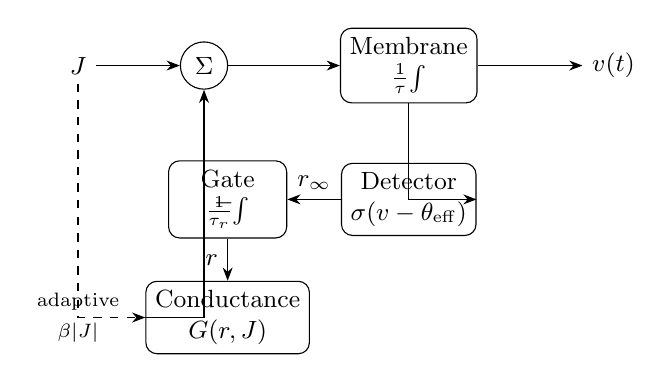
\begin{tikzpicture}[
      >=Stealth, font=\small,
      block/.style={draw, rounded corners, minimum width=15mm, minimum height=8mm, align=center},
      sum/.style={draw, circle, minimum size=6mm, inner sep=0pt}]
    \node (in) at (0,0) {$J$};
    \node[sum] (sum) at (1.6,0) {$\Sigma$};
    \node[block] (mem) at (4.2,0) {Membrane\\ $\tfrac{1}{\tau}\!\int$};
    \node (out) at (6.8,0) {$v(t)$};
    \draw[->] (in) -- (sum);
    \draw[->] (sum) -- (mem);
    \draw[->] (mem) -- (out);
    \node[block] (det) at (4.2,-1.7) {Detector\\ $\sigma(v-\teff)$};
    \node[block] (gate) at (1.9,-1.7) {Gate\\ $\tfrac{1}{\tau_r}\!\int$};
    \node[block] (cond) at (1.9,-3.2) {Conductance\\ $G(r,J)$};
    \draw[->] ($(mem.south)$) |- (det.east);
    \draw[->] (det) -- (gate) node[midway,above]{$\rinf$};
    \draw[->] (gate) -- node[left]{$r$} (cond);
    \draw[->] (cond) -| (sum) node[pos=0.75,right]{$-$};
    \draw[->, dashed] (in) |- ($(cond.west)+(-0.0,0)$);
    \node[align=center] at (0.0,-3.2) {\scriptsize adaptive\\ \scriptsize $\beta|J|$};
  \end{tikzpicture}}
  \caption{Signal flow of the (Adaptive) HyperLIF neuron as implemented. The
  forward path integrates the membrane; the feedback loop
  (detector $\to$ gate $\to$ conductance) implements the continuous reset through
  $r(t)$. The dashed feedforward path is the adaptive term $\beta|J|$ that scales
  the reset conductance with input magnitude (\cref{eq:adaptive-gain}); removing
  it recovers the fixed-gain HyperLIF.}
  \label{fig:schematic}
\end{figure}

% ===========================================================================
\section{Results}\label{sec:results}
% ===========================================================================

\subsection{Continuous vs.\ Hard Reset}\label{sec:results-step}
\Cref{fig:step} contrasts LIF and HyperLIF under the same current step. The LIF
membrane produces the familiar saw-tooth of hard resets, whereas the HyperLIF
membrane rises smoothly, hovers near threshold, and is discharged continuously
by the gate. A revealing detail is that the gate completes several
readiness cycles while only a single upward threshold crossing is registered:
the continuous reset keeps the trajectory near, but mostly below, the event
level, so the event channel under-reports the activity that the gate state makes
explicit. This already motivates treating $r(t)$ as an observable in its own
right (\Cref{sec:readiness}).

\begin{figure}[t]
  \centering
  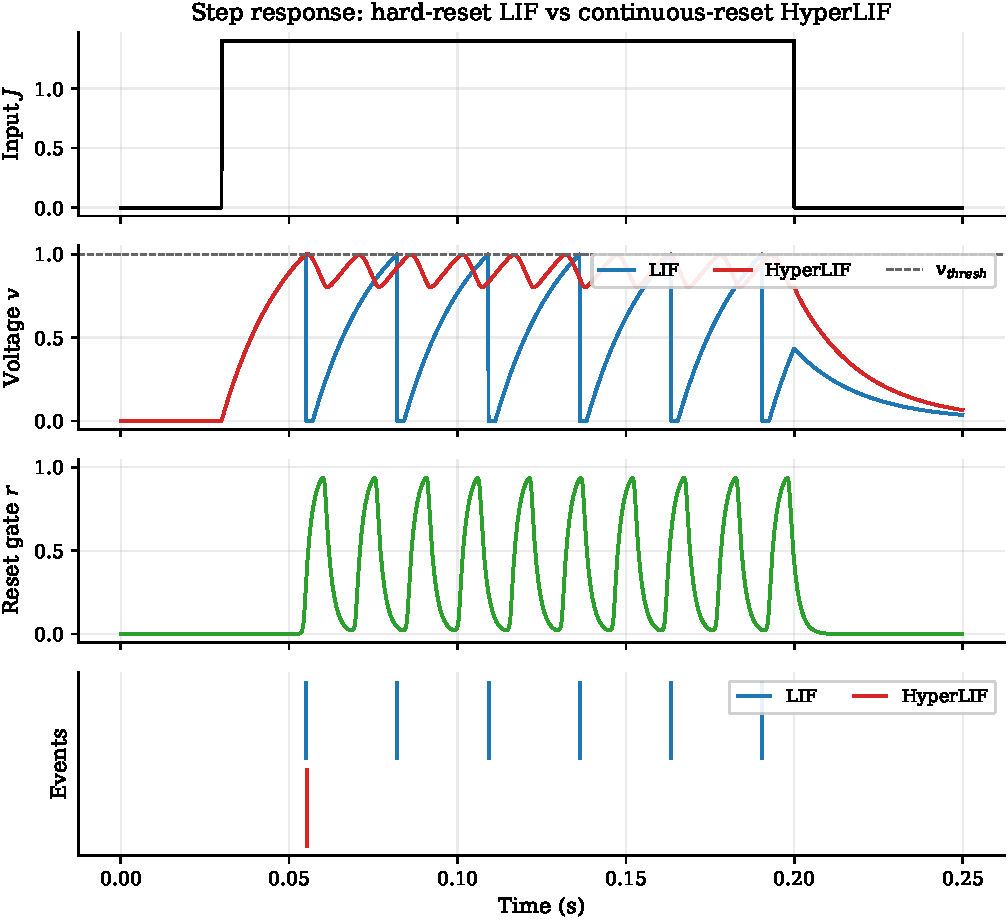
\includegraphics[width=\columnwidth]{fig_step}
  \caption{Step response. Hard-reset LIF (blue) vs.\ continuous-reset HyperLIF
  (red): input current, membrane voltage with threshold, the HyperLIF reset gate
  $r(t)$, and event rasters. The gate cycles several times while only one
  HyperLIF event is registered. Source: \code{01\_lif\_vs\_hyperlif.csv}.}
  \label{fig:step}
\end{figure}

\subsection{Fixed vs.\ Adaptive Reset Conductance}\label{sec:results-stress}
\Cref{fig:stress} drives both continuous-reset models with a stress current that
ramps to $J=4$. During the high-current phase the fixed-gain HyperLIF membrane
latches above threshold (its gate saturates and its conductance plateaus at
$\Gb=100$), i.e.\ it enters the DB. Adaptive HyperLIF instead raises its
conductance with $|J|$ (the dynamic gain $\Gdyn$ tracks the staircase input) and
keeps oscillating below threshold. This is the time-domain signature of the
operating-range expansion characterized statically next.

\begin{figure}[t]
  \centering
  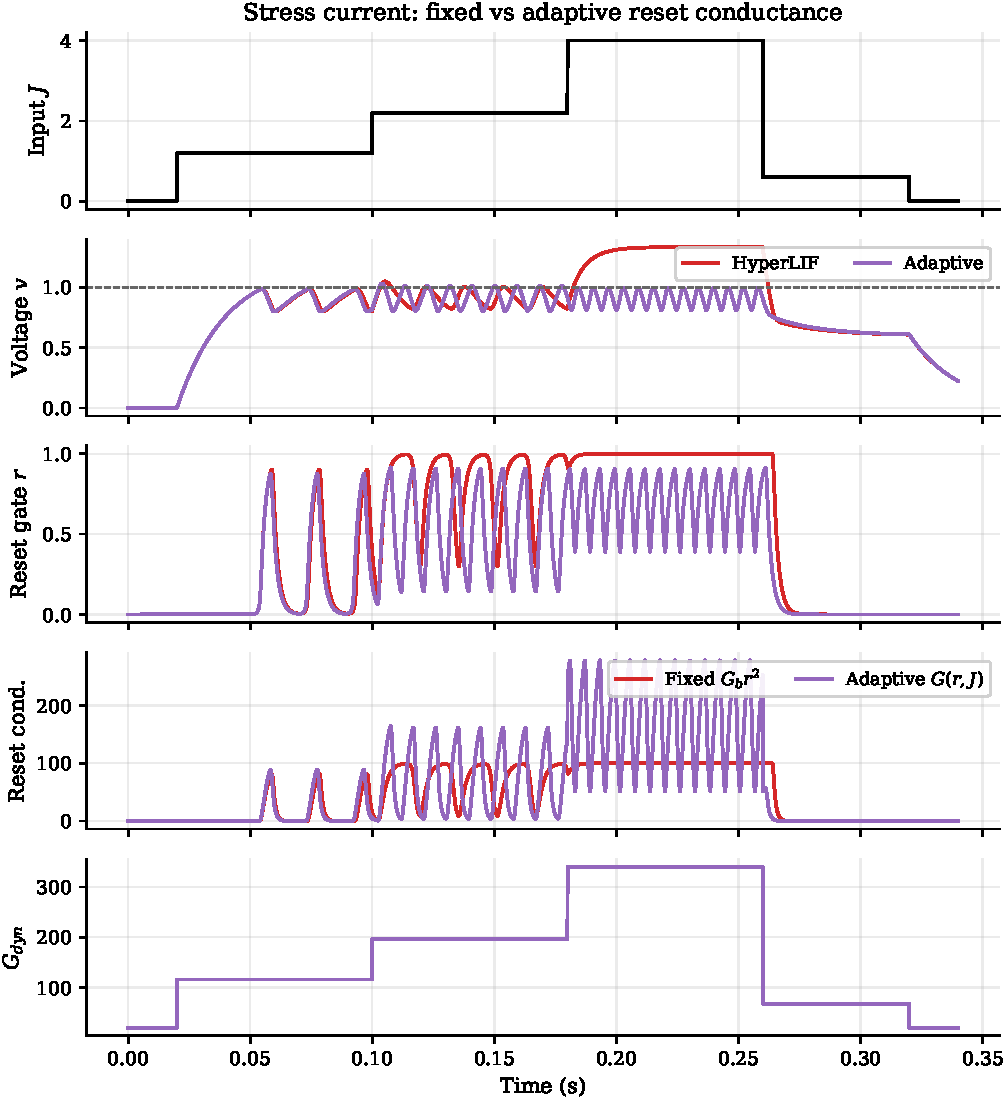
\includegraphics[width=\columnwidth]{fig_stress}
  \caption{Stress current. Fixed-gain HyperLIF (red) latches during the
  high-current phase while Adaptive HyperLIF (purple) sustains oscillation; the
  dynamic gain $\Gdyn=\Gbase+\beta|J|$ follows the input staircase. Source:
  \code{02\_hyperlif\_vs\_adaptive.csv}.}
  \label{fig:stress}
\end{figure}

\subsection{Frequency--Current Response and the Depolarization Block}
\label{sec:results-fi}
\Cref{fig:fi} and \Cref{tab:sweep} summarize the steady-state response to
constant current. Three regimes are evident. LIF firing increases monotonically
and without bound (runaway). Fixed-gain HyperLIF fires only over a narrow band
($J\in[1.5,2.2]$) and then collapses to zero at $J\approx 2.3$--$2.4$, close to
the open-gate branch estimate $\Jdb=2.4$ from \cref{eq:jdb}; beyond it the mean membrane
voltage climbs linearly as $v^\ast=J/(1+\tau\Gb)=J/3$ (e.g.\ $1.000$ at $J=3$,
$1.333$ at $J=4$), and the gate saturates---the high-voltage latch of
\cref{eq:vstar}. The fixed-point prediction matches the simulated latched voltage
to all reported digits ($1.3333$ vs.\ $1.3333$ at $J=4$). Adaptive HyperLIF fires
over a substantially wider band ($J\in[1.6,3.5]$) with a higher peak rate
($151$ vs.\ $73\,$Hz) and a \emph{bounded} mean voltage near $0.9$, never
exhibiting the high-voltage latch, consistent with \cref{eq:vinf,eq:beta-crit}
($v^\ast_\infty=0.625<0.8$). The adaptive model is not unconditionally
firing: with finite $\beta$ it has its own, higher operating ceiling
($J\gtrsim 3.6$ here) above which the bounded oscillation no longer crosses the
default event surface and detected spiking ceases. Crucially, this failure is
bounded---the membrane oscillates below threshold near $0.9$ rather than
latching at $J/3$---so the event channel becomes silent while the continuous
state remains dynamically active.

\begin{figure}[t]
  \centering
  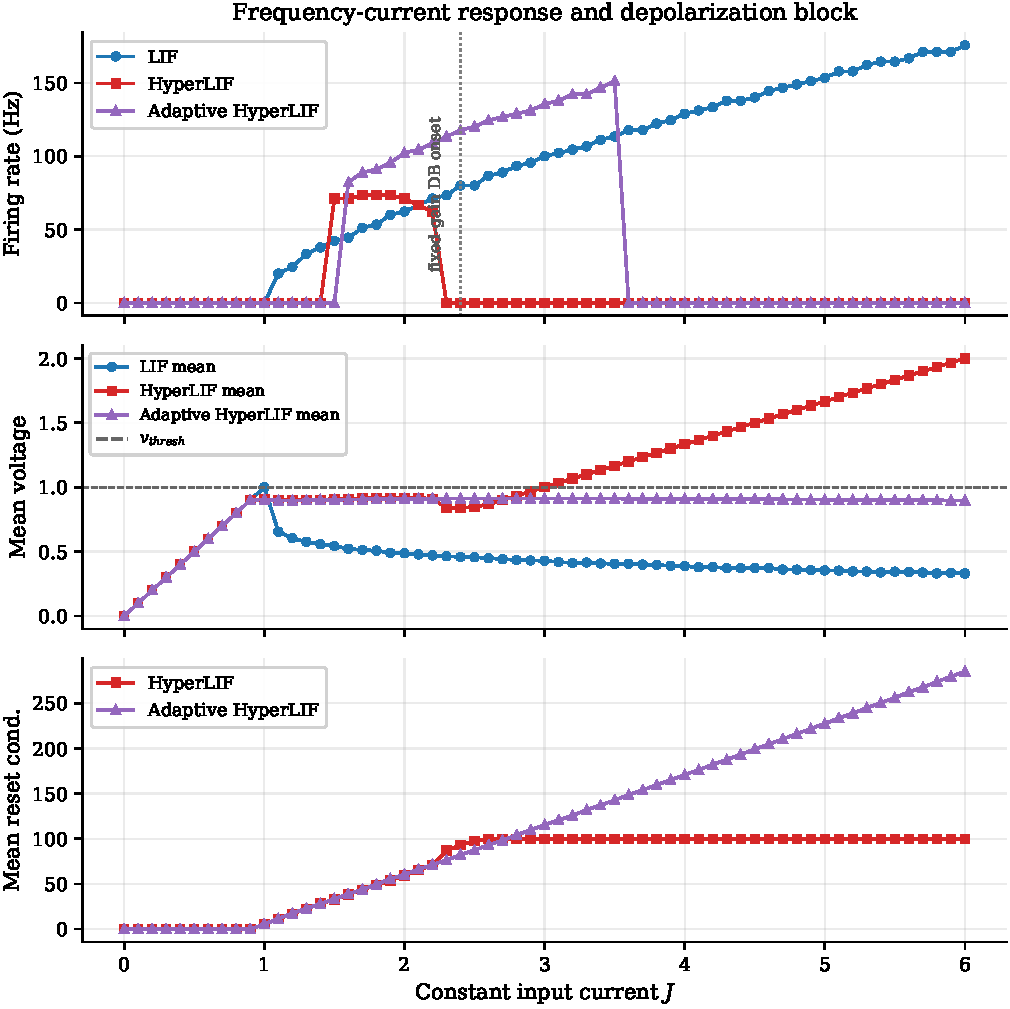
\includegraphics[width=\columnwidth]{fig_fi}
  \caption{Frequency--current response. (Top) firing rate: LIF runs away,
  fixed-gain HyperLIF collapses near the open-gate branch estimate $\Jdb=2.4$, Adaptive
  HyperLIF sustains a wider band. (Middle) mean voltage: the HyperLIF latch
  climbs as $J/3$ while Adaptive stays bounded near $0.9$. (Bottom) mean reset
  conductance saturates for HyperLIF but grows with $J$ for Adaptive. Source:
  \code{03\_current\_sweep.csv}.}
  \label{fig:fi}
\end{figure}

\begin{table}[t]
\centering
\caption{Steady-state response at representative constant currents (from
\code{03\_current\_sweep.csv}). The fixed-gain HyperLIF firing rate collapses to
zero and its mean voltage latches above threshold once $J$ exceeds the analytical
depolarization-block onset $\Jdb=2.4$, whereas Adaptive HyperLIF sustains spiking
with a bounded mean voltage.}
\label{tab:sweep}
\footnotesize
\begin{tabular}{@{}cccccc@{}}
\toprule
& \multicolumn{3}{c}{Firing rate (Hz)} & \multicolumn{2}{c}{Mean voltage} \\
\cmidrule(lr){2-4}\cmidrule(lr){5-6}
$J$ & LIF & HyperLIF & Adaptive & HyperLIF & Adaptive \\
\midrule
1.0 & 0.0   & 0.0  & 0.0   & 0.906 & 0.906 \\
1.5 & 42.2  & 71.1 & 0.0   & 0.908 & 0.903 \\
2.0 & 62.2  & 71.1 & 102.2 & 0.917 & 0.910 \\
2.4 & 80.0  & 0.0  & 117.8 & 0.840 & 0.912 \\
3.0 & 100.0 & 0.0  & 135.6 & 1.000 & 0.913 \\
4.0 & 128.9 & 0.0  & 0.0   & 1.333 & 0.910 \\
\bottomrule
\end{tabular}
\end{table}

\Cref{fig:db} isolates the contrast at a single sustained drive $J=3.3$ (above
$\Jdb$): the fixed-gain neuron settles to the predicted latched voltage $1.1$
with a saturated gate and emits no further events, while the adaptive neuron
produces a clean limit cycle with $42$ events over $0.3\,$s.

\begin{figure}[t]
  \centering
  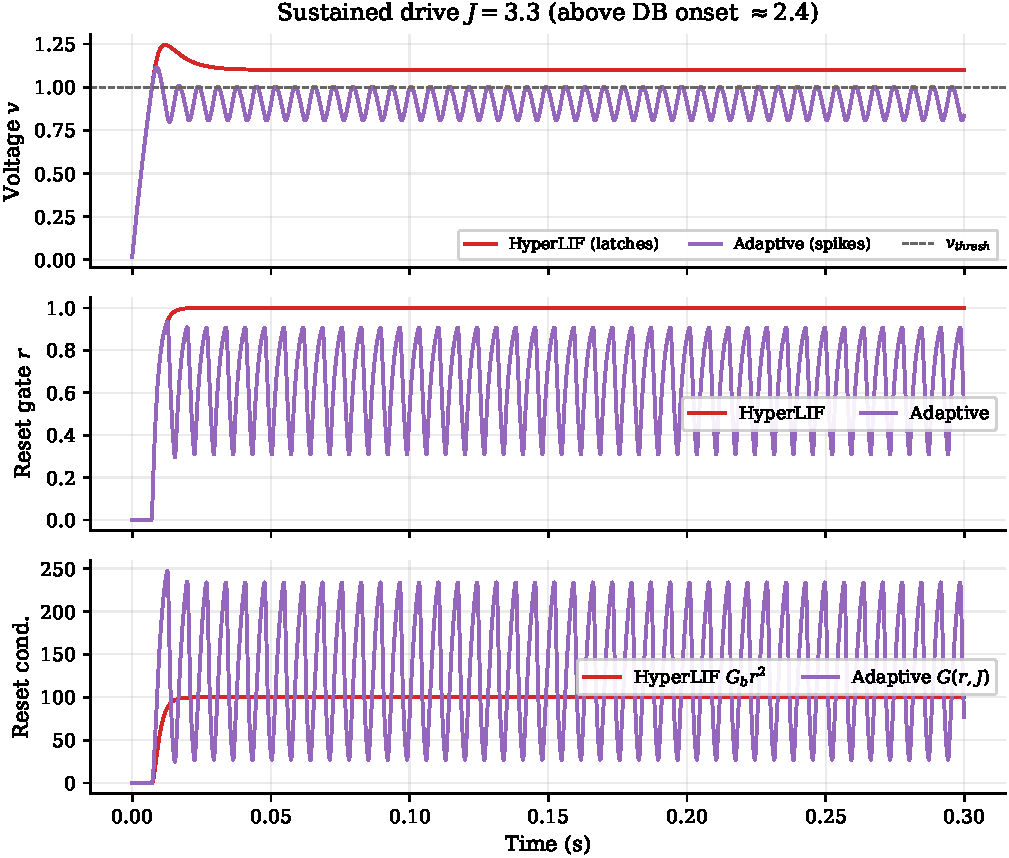
\includegraphics[width=\columnwidth]{fig_db}
  \caption{Depolarization-block latch at sustained drive $J=3.3$. Fixed-gain
  HyperLIF (red) latches at $v\approx 1.1$ with a saturated gate; Adaptive
  HyperLIF (purple) maintains a limit cycle. Source:
  \code{04\_depolarization\_block.csv}.}
  \label{fig:db}
\end{figure}

\subsection{Numerical Accuracy and Stability}\label{sec:results-integration}
\Cref{fig:integration} and \Cref{tab:integration} report the membrane error of
both stepping schemes against the RK4 reference. Both converge at first order in
$\Delta t$, and the gate error is identical because the gate update
\cref{eq:gate-update} is shared. In the convergent regime the explicit and
exponential schemes have comparable accuracy (here the explicit scheme has a
slightly lower trajectory RMSE), so the value of the exponential scheme is not
accuracy but \emph{stability}: \Cref{fig:integration}(b) drives the gate fully
open ($J=4$, $\lambda\approx 150$) and increases $\Delta t$; once
$\lambda\Delta t>2$ the explicit scheme develops growing spurious overshoot
(its maximum $|v|$ rises to $2,3,4,6$ as $\lambda\Delta t$ grows), whereas the
exponential scheme remains bounded near the true latched value $v^\ast=J/3$. This
is why the Nengo port, which must remain well-behaved at arbitrary $\Delta t$ and
high conductance, uses the exponential update.

\begin{figure}[t]
  \centering
  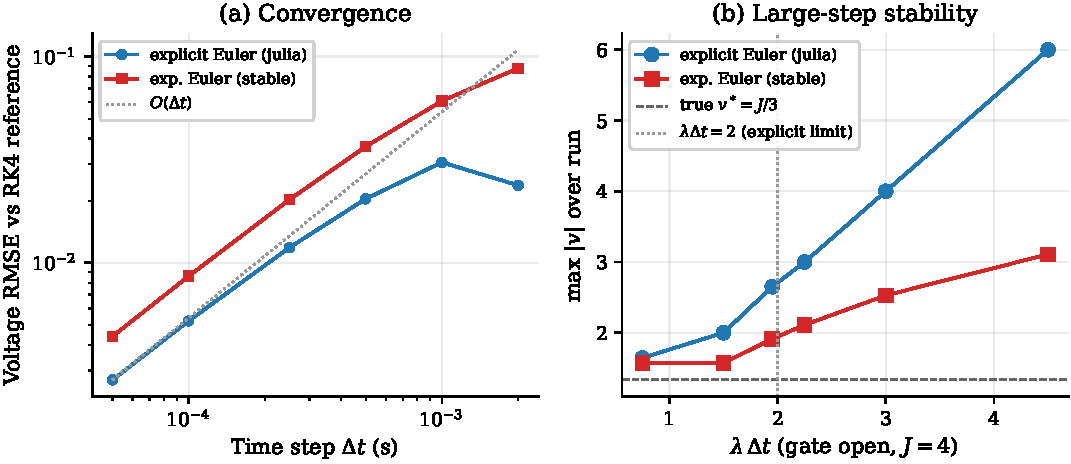
\includegraphics[width=\columnwidth]{fig_integration}
  \caption{(a) First-order convergence of both schemes against an RK4 reference
  of the continuous ODE. (b) Large-step stability at $J=4$: explicit Euler
  overshoots once $\lambda\Delta t>2$; the exponential update stays bounded near
  $v^\ast=J/3$. Source: \code{06\_integration\_accuracy.csv},
  \code{06\_stability.csv}.}
  \label{fig:integration}
\end{figure}

\begin{table}[t]
\centering
\caption{Voltage error of the two stepping schemes against a fine RK4 reference
of the continuous ODE (from \code{06\_integration\_accuracy.csv}). Both converge
at first order; the gate update is shared and identical.}
\label{tab:integration}
\footnotesize
\begin{tabular}{@{}cccc@{}}
\toprule
$\Delta t$ (s) & RMSE explicit & RMSE exponential & Gate RMSE \\
\midrule
$2.000\times10^{-3}$ & 0.0237  & 0.0877  & 0.16   \\
$1.000\times10^{-3}$ & 0.0307  & 0.0609  & 0.2    \\
$5.000\times10^{-4}$ & 0.0204  & 0.0366  & 0.134  \\
$2.500\times10^{-4}$ & 0.0118  & 0.0202  & 0.0806 \\
$1.000\times10^{-4}$ & 0.00522 & 0.0086  & 0.0367 \\
$5.000\times10^{-5}$ & 0.0027  & 0.00439 & 0.0191 \\
\bottomrule
\end{tabular}
\end{table}

\subsection{Python--Nengo Parity}\label{sec:results-parity}
\Cref{fig:parity} and \Cref{tab:parity} report the central validation result.
The standalone exponential stepping and the Nengo custom-neuron stepping produce
identical voltage and gate traces, and identical event timing, for both models
and both protocols: the voltage and gate RMSE are exactly $0$, the maximum
absolute voltage/gate difference is exactly $0$, and the event-mismatch count is
$0$. The difference trace in \Cref{fig:parity} is flat at the $10^{-15}$ scale.
Because both implementations call the same numerical kernel
(\Cref{sec:nengo}), this is an algorithmic identity, not a statistical fit---the
strongest form of evidence that the Nengo port \emph{is} the implemented model
rather than an approximation of it.

\begin{figure}[t]
  \centering
  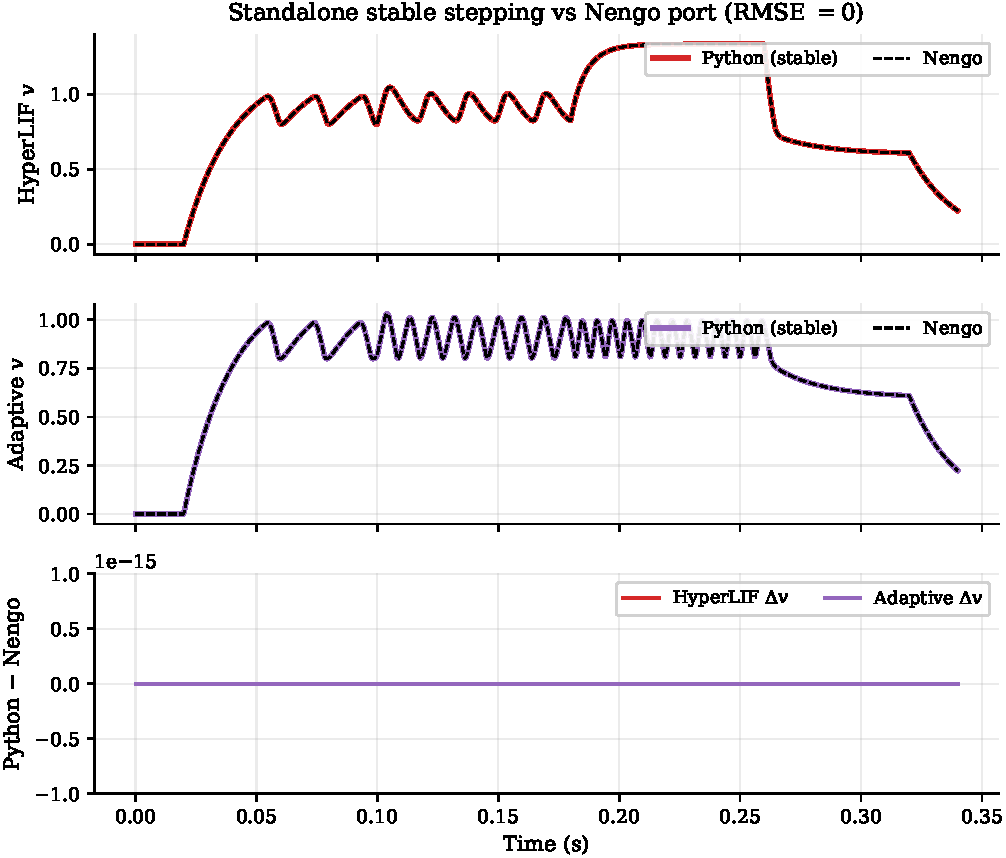
\includegraphics[width=\columnwidth]{fig_parity}
  \caption{Standalone stable stepping (thick colored) vs.\ the Nengo port
  (dashed black) for HyperLIF and Adaptive HyperLIF voltage, with the difference
  trace (bottom) flat at machine precision. Source:
  \code{07\_python\_vs\_nengo.csv}, \code{07\_parity\_metrics.csv}.}
  \label{fig:parity}
\end{figure}

\begin{table}[t]
\centering
\caption{Standalone stable stepping vs.\ the Nengo \code{NeuronType} port (from
\code{07\_parity\_metrics.csv}). Agreement is exact to floating point: zero RMSE,
zero maximum voltage/gate difference, and zero event-timing mismatches across
both protocols and both models.}
\label{tab:parity}
\footnotesize
\begin{tabular}{@{}llcccc@{}}
\toprule
Model & Protocol & $v$ RMSE & $\max|\Delta v|$ & $r$ RMSE & Event mism. \\
\midrule
HyperLIF & stress & 0 & 0 & 0 & 0 \\
Adaptive & stress & 0 & 0 & 0 & 0 \\
HyperLIF & step   & 0 & 0 & 0 & 0 \\
Adaptive & step   & 0 & 0 & 0 & 0 \\
\bottomrule
\end{tabular}
\end{table}

\subsection{Gate-State Decoding}\label{sec:results-decode}
\Cref{fig:decode} and \Cref{tab:decoding} compare scalar linear decoders fit to
three internal signals of an Adaptive HyperLIF neuron driven by a smooth current.
A voltage decoder recovers the input current with test RMSE $0.258$; a decoder of
exponentially filtered events does worse ($0.321$), reflecting the sparsity of
the event channel; and a decoder of the reset gate recovers a readiness target
with test RMSE $0.287$. The gate decoder is comparable to the voltage decoder
even though the raw gate is a fast, spiky signal, indicating that the gate
carries genuine, decodable information about proximity to the reset transition.

\begin{figure}[t]
  \centering
  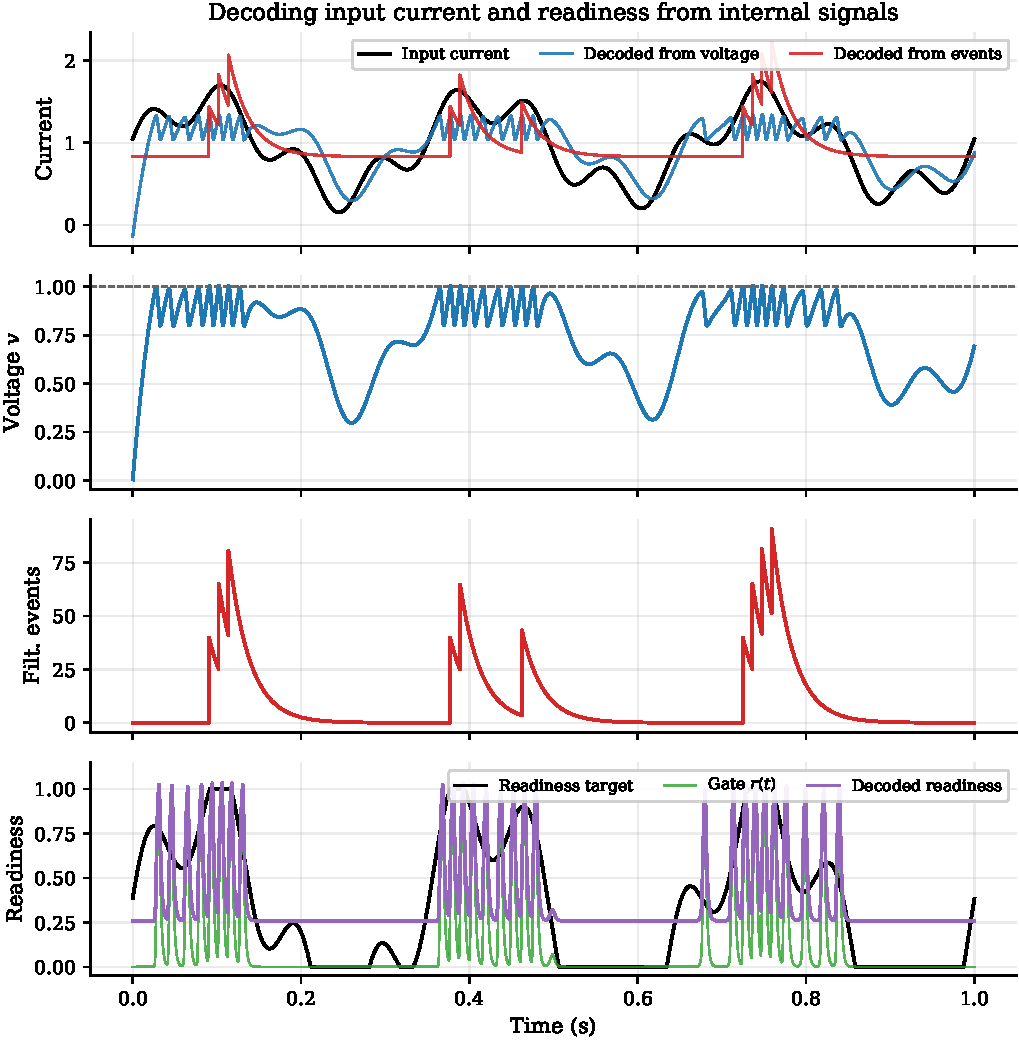
\includegraphics[width=\columnwidth]{fig_decode}
  \caption{Decoding from internal signals. (Top) input current and its linear
  decodes from voltage and from filtered events. (Middle panels) the voltage and
  filtered-event features. (Bottom) the readiness target, the raw gate $r(t)$,
  and the gate-based readiness decode. Source:
  \code{05\_gate\_state\_decoding.csv}, \code{05\_decoding\_metrics.csv}.}
  \label{fig:decode}
\end{figure}

\begin{table}[t]
\centering
\caption{Scalar linear decoders fit by least squares with a 70/30 train/test
split (from \code{05\_decoding\_metrics.csv}).}
\label{tab:decoding}
\footnotesize
\begin{tabular}{@{}lcc@{}}
\toprule
Decoder & Train RMSE & Test RMSE \\
\midrule
Voltage $\to$ input current        & 0.293 & 0.258 \\
Filtered events $\to$ input current & 0.347 & 0.321 \\
Reset gate $\to$ readiness         & 0.283 & 0.287 \\
\bottomrule
\end{tabular}
\end{table}

% ===========================================================================
\section{Interpretation: Gate-State Readiness-to-Fire}\label{sec:readiness}
% ===========================================================================
The reset gate is more than an internal bookkeeping variable. By
\cref{eq:theta,eq:sigmoid}, $r$ tracks $\sigma(\alpha(v-(\vth-\gamma r)))$: it
rises as the membrane approaches the (hysteresis-lowered) threshold and saturates
once the reset trajectory is committed. It is therefore a continuous
\emph{readiness-to-fire} signal: small $r$ means far from the reset transition,
rising $r$ means approaching it, and saturated $r$ means the reset is fully
engaged. Two observations from \Cref{sec:results} make this concrete. First, in
\Cref{fig:step} the gate completes several readiness cycles while the event
channel reports a single spike---the gate exposes sub-threshold structure that
spikes discard. Second, \Cref{tab:decoding} shows that a linear gate decoder is
competitive with a voltage decoder for a readiness target. Unlike the voltage,
whose interpretation near reset is ambiguous in a hard-reset neuron, the gate is
a bounded $[0,1]$ quantity with a direct interpretation in terms of the effective
threshold. This makes $r(t)$ a natural \emph{residual feature} to augment
spike/rate features in downstream estimation.

% ===========================================================================
\section{Connection to Residual Augmentation and Quaternion Attitude Control}
\label{sec:bridge}
% ===========================================================================
We now outline the intended application, and we are explicit that this section
is \emph{forward-looking}: no closed-loop control results are claimed here. The
NEF pipeline that Nengo implements suggests a direct route to using HyperLIF
neurons inside an attitude controller. An attitude error---for example a
quaternion error vector between the estimated and desired
orientations~\cite{markley2014attitude}---is encoded as input current $J$ to a
HyperLIF ensemble; the ensemble's spikes, membrane voltages, and reset gates are
decoded into control or residual features; and a controller maps those features
to torques. NEF-based spiking networks have already been shown to learn adaptive
control signals online~\cite{dewolf2016reach}, and the gate provides an
additional, interpretable channel:
\begin{equation}
  \text{error} \to J \to (v, r, \text{spikes}) \to \text{decoded residual} \to \text{torque}.
  \label{eq:pipeline}
\end{equation}
The hypothesis to be tested in future work is that a gate-state residual term
improves tracking or robustness relative to spike-only or voltage-only decoding,
because $r(t)$ encodes readiness information that the event channel omits
(\Cref{sec:readiness}). The validated \code{NeuronType} port and the exact
parity result of \Cref{sec:results-parity} are precisely what make such a study
trustworthy: any controller behavior can be attributed to the model, not to an
implementation discrepancy. The present paper deliberately keeps the neuron
reference free of controller code; the controller stage will import this
reference rather than re-define the equations.

% ===========================================================================
\section{Limitations}\label{sec:limitations}
% ===========================================================================
We list the limitations plainly. (i) The validation is performed on a single
neuron driven by injected current; ensemble-level NEF decoding and closed-loop
control are not evaluated here. (ii) The parameters in \Cref{tab:params} are a
normalized reference set chosen for clean demonstration; they differ from the
benchmark-scale training parameters of~\cite{hyperlif_theory}, so the specific
numbers ($\Jdb=2.4$, $\beta_{\mathrm{crit}}=62.5$, etc.) are parameter-dependent
instances of the general relations \cref{eq:jdb,eq:beta-crit}, not universal
constants. (iii) The DB analysis uses a frozen-gate fixed-point argument; it
correctly predicts the onset and latched voltage observed in simulation but is a
sufficient-condition characterization rather than a full bifurcation analysis,
and the adaptive ceiling above $J\approx 3.6$ is reported empirically. (iv) The
decoders are deliberately simple scalar least-squares fits on a single neuron;
the raw gate is spiky and its decode is correspondingly noisy. (v) The
attitude-control connection of \Cref{sec:bridge} is a design and a hypothesis,
not a result. (vi) The explicit-Euler scheme, included for reference fidelity,
is only conditionally stable (\Cref{sec:results-integration}).

% ===========================================================================
\section{Future Work}\label{sec:future}
% ===========================================================================
The natural next steps are: (a) NEF ensemble experiments---tuning-curve
calibration, multi-neuron encoding/decoding, and noise robustness for the gate
channel; (b) closed-loop quaternion attitude control following
\cref{eq:pipeline}, with ablations isolating spike-only, voltage-only,
gate-only, and combined decoders; (c) repeated, seed-matched trials with
paper-scale statistics; (d) mapping the gate $r(t)$ to local, multi-factor
plasticity rules as a low-memory alternative to backpropagation through time, as
suggested in~\cite{hyperlif_theory}; and (e) deployment considerations on
event-driven neuromorphic hardware~\cite{davies2018loihi}, where the intrinsic
activity bounding of the adaptive model is attractive.

% ===========================================================================
\section{Conclusion}\label{sec:conclusion}
% ===========================================================================
We presented a clean, equation-faithful, and rigorously validated reference
implementation of the HyperLIF and Adaptive HyperLIF continuous-reset neurons,
compatible with Nengo. Every manuscript equation is realized in code; a
frozen-open-gate analysis gives the branch estimate
$\Jdb=(\vth-\gamma)(1+\tau\Gb)$ and branch voltage $J/(1+\tau\Gb)$; the latter
matches the simulated high-drive latch. The adaptive conductance law bounds the
positive-drive, $r=1$ asymptotic branch below the gate knee when
$\beta>1/(\tau(\vth-\gamma))$, changing the high-drive regime without proving
global stability or indefinite firing. The two stepping schemes
are characterized for accuracy and stability; and the Nengo port reproduces the
standalone model to floating-point exactness. Interpreting the reset gate as a
decodable readiness-to-fire signal, we outlined a concrete, validated-substrate
path toward gate-state residual decoding for quaternion attitude control, which
we leave as future work. The complete project regenerates every figure, table,
and number from the included code and data.

% ===========================================================================
\appendices
\section{Parameters}\label{app:params}
\Cref{tab:params} lists the default parameters, reflected directly from the
\code{LIFParams}, \code{HyperLIFParams}, and \code{AdaptiveHyperLIFParams}
dataclasses, so the table cannot drift from the implementation.

\begin{table}[t]
\centering
\caption{Default parameters of the reference implementation, reflected directly
from the \code{LIFParams}, \code{HyperLIFParams}, and
\code{AdaptiveHyperLIFParams} dataclasses. All voltages and gains are in the
normalized convention ($\vr=\vre=0$, $\vth=1$); $J$ and $G$ are dimensionless
relative to the leak.}
\label{tab:params}
\footnotesize
\begin{tabular}{@{}lcccc@{}}
\toprule
Parameter & Symbol & LIF & HyperLIF & Adaptive \\
\midrule
Membrane time constant & $\tau$ (s)             & 0.02  & 0.02  & 0.02 \\
Refractory period      & $\tau_{\mathrm{ref}}$ (s) & 0.002 & --    & --   \\
Resting potential      & $\vr$                  & 0     & 0     & 0    \\
Reset potential        & $\vre$                 & 0     & 0     & 0    \\
Threshold              & $\vth$                 & 1     & 1     & 1    \\
Gate steepness         & $\alpha$               & --    & 100   & 100  \\
Gate time constant     & $\tau_r$ (s)           & --    & 0.002 & 0.002 \\
Hysteresis factor      & $\gamma$               & --    & 0.2   & 0.2  \\
Fixed reset gain       & $\Gb$                  & --    & 100   & --   \\
Baseline reset gain    & $\Gbase$               & --    & --    & 20   \\
Adaptive scaling       & $\beta$                & --    & --    & 80   \\
Spike amplitude        & $A$                    & 1     & 1     & 1    \\
Min.\ voltage clamp    & $\vmin$                & 0     & 0     & 0    \\
\bottomrule
\end{tabular}
\end{table}

\section{Equation-to-Code Map}\label{app:map}
\Cref{eq:lif-ode,eq:lif-update} correspond to \code{src/neurons/lif.py}
(\code{\_lif\_voltage\_update}, \code{simulate\_lif}).
\Cref{eq:theta,eq:sigmoid,eq:gate-ode,eq:hyperlif-ode,eq:gate-update,%
eq:stable-update,eq:euler-update} correspond to \code{src/neurons/hyperlif.py}
(\code{gate\_target}, \code{exact\_gate\_update}, \code{stable\_voltage\_update},
\code{HyperLIFNeuron.step}).
\Cref{eq:adaptive-gain,eq:adaptive-ode} correspond to
\code{src/neurons/adaptive\_hyperlif.py}.
The Nengo realization of \Cref{alg:step} is in
\code{src/neurons/nengo\_hyperlif.py} (\code{HyperLIFNengo.step},
\code{AdaptiveHyperLIFNengo.step}).
\Cref{eq:vstar,eq:jdb,eq:vinf,eq:beta-crit} are implemented and validated in
\code{src/analysis/depolarization\_block.py} and exercised by
\code{experiments/03\_current\_sweep.py}. A line-level table is maintained in
the accompanying \code{MATH\_CODE\_MAP.md}.

\section{Reproducibility}\label{app:repro}
From the project root, after creating the environment
(\code{scripts/setup\_env.ps1}): run \code{python experiments/run\_all.py},
\code{python figures/make\_figures.py}, \code{python tables/make\_tables.py}, and
\code{scripts/build\_paper.ps1}. This regenerates all CSV/logs, all figures
(PNG\,+\,PDF), all \LaTeX{} tables, and compiles this document. See
\code{REPRODUCIBILITY.md} and \code{RUNNERS.md} for details and
\code{RESULTS\_AUDIT.md} for the validated/exploratory and
paper-ready/future-work classification of every claim.

% ===========================================================================
\bibliographystyle{IEEEtran}
\bibliography{references}

\end{document}
